\documentclass[10pt, letterpaper]{report}
% !TeX program = xelatex
%==================PREAMBOLO=======================%
\usepackage[utf8]{inputenc}
\usepackage{psvectorian}
\usepackage{pgfplots}
\usepackage[Rejne]{fncychap}
\usepackage[export]{adjustbox}
\usepackage[T1]{fontenc}
\usepackage{lmodern}
\usepackage[shortlabels]{enumitem}
\usepackage{moresize}
\usepackage{graphicx} % Required for inserting images
\usepackage{hyperref}
\usepackage{listings}
\usepackage[table,xcdraw]{xcolor}
\usepackage{amssymb}
\usepackage{amsmath}
\usepackage[italian]{babel}
\usepackage{nicefrac, xfrac}
\usepackage{tikz}
\usepackage{mathrsfs} 
\usepackage{titletoc}
\usepackage{fancyhdr}
\usepackage{psvectorian,lipsum}
\usepackage{fourier-orns}
\usepackage{lipsum}
\usepackage[paper=a4paper,left=25mm,right=25mm,bottom=25mm,top=25mm]{geometry}
\definecolor{light-gray}{gray}{0.95}
\definecolor{cop}{HTML}{f7ecd7}
\definecolor{copAut}{HTML}{ababab}
\definecolor{copAut2}{HTML}{c3c3e6}
\definecolor{purcop}{HTML}{d0d3db}
\definecolor{sapienza}{HTML}{660f1d}
\definecolor{lightSapienza}{HTML}{e3d3d5}
\definecolor{darkgreen}{HTML}{008000}
\definecolor{cartaRiciclata}{HTML}{fcfcf7}
\newcommand{\redText}[1]{\color{red}#1\color{black}}
\newcommand{\code}[1]{\colorbox{light-gray}{\texttt{#1}}}
\newcommand{\codee}[1]{\colorbox{white}{\texttt{#1}}}
\newcommand{\K}{{\mathbb K}}
\newcommand{\notimplies}{%
  \mathrel{{\ooalign{\hidewidth$\not\phantom{=}$\hidewidth\cr$\implies$}}}}
\newcommand{\flowerLine}{ \begin{center}\decofourleft\hphantom{ }\decoone\hphantom{ }\decofourright\hphantom{}\hphantom{aa}
\decofourleft\hphantom{ }\decoone\hphantom{ }\decofourright\hphantom{}\hphantom{aa}
\decofourleft\hphantom{ }\decoone\hphantom{ }\decofourright\hphantom{}\hphantom{aa}
\decofourleft\hphantom{ }\decoone\hphantom{ }\decofourright\hphantom{}\hphantom{aa} 
\decofourleft\hphantom{ }\decoone\hphantom{ }\decofourright\hphantom{}\hphantom{aa}
\decofourleft\hphantom{ }\decoone\hphantom{ }\decofourright\hphantom{}\hphantom{aa}
\decofourleft\hphantom{ }\decoone\hphantom{ }\decofourright\hphantom{}\hphantom{aa}
\decofourleft\hphantom{ }\decoone\hphantom{ }\decofourright\hphantom{}\hphantom{aa}
\decofourleft\hphantom{ }\decoone\hphantom{ }\decofourright\hphantom{}\hphantom{aa}
\end{center}}
\definecolor{g}{RGB}{60, 50, 50}
\newcommand{\textg}[1]{\color{g}{\textbf{#1}}\color{black}}
\newcommand{\teo}[1]{{\large\color{sapienza}\textbf{Teorema #1 :\hphantom{a}}}}
\newcommand{\defi}[1]{{\large\color{sapienza}\textbf{Definizione #1 :\hphantom{a}}}}
\newcommand{\claim}[1]{{\color{sapienza}\textbf{Claim #1 :\hphantom{a}}}}
\newcommand{\lemma}[1]{{\color{sapienza}\textbf{Lemma #1 :\hphantom{a}}}}
\newcommand{\dimo}[1]{{\color{sapienza}\textbf{Dimostrazione #1 :\hphantom{a}}}}
\newcommand{\prop}[1]{{\color{sapienza}\textbf{Proposizione #1 :\hphantom{a}}}}
\newcommand\greybox[1]{%
  \vskip\baselineskip%
  \par\noindent\colorbox{light-gray}{%
    \begin{minipage}{\textwidth}#1\end{minipage}%
  }%
  \vskip\baselineskip%
}
\newcommand\sapbox[1]{%
  \vskip\baselineskip%
  \par\noindent\colorbox{lightSapienza}{%
    \begin{minipage}{\textwidth}#1\end{minipage}%
  }%
  \vskip\baselineskip%
}

\newcommand{\Z}{{\mathbb Z}}
\newcommand{\blank}{{\sqcup}}
\newcommand{\R}{{\mathbb R}}
\newcommand{\N}{{\mathbb N}}
\newcommand{\C}{{\mathbb C}}
\newcommand{\Sn}{{\mathcal S_n}}
\newcommand{\An}{{\mathcal A_n}}
\newcommand{\E}{{\mathcal E}}
\newcommand{\B}{{\mathcal B}}
\newcommand{\mcm}{{\text{mcm}}}
\newcommand{\rg}{{\text{rg}}}
\newcommand{\ve}{{\bar v}}
\newcommand{\spaz}{{\text{\hphantom{aa}}}}
\newcommand{\MCD}{{\text{MCD}}}
\newcommand{\tc}{{\text{ tale che }}}
\newcommand{\supp}{{\text{Supp}}}
\newcommand{\acc}{\\\hphantom{}\\}
\newcommand{\aut}{{\text{Aut}}}
\newcommand{\Span}{{\text{Span}}}
\newcommand{\End}{{\text{End}}}
\newcommand{\cen}{{\text{Centro}}}
\newcommand{\norm}{{\unlhd}}
\newcommand{\ciclS}{{\left \langle }}
\newcommand{\ciclE}{{\right \rangle }}
\newcommand{\boxedMath}[1]{\begin{tabular}{|c|}\hline \texttt{#1} \\ \hline\end{tabular} :}
\newcommand{\shell}[1]{\colorbox{black}{\textcolor{white}{\texttt{#1}}}}
\newcommand{\eqImportante}[1]{\begin{center}\huge\lefthand\hphantom{a}
    \normalsize\texttt{#1}
    \hphantom{aaa}\huge\righthand\end{center}}

\fancyhf{}
\pagestyle{fancy}
\usepackage{pgf-pie}  
\usetikzlibrary{positioning}

\renewcommand{\headrule}{%
\vspace{-8pt}\hrulefill
\raisebox{-2.1pt}{\quad\decothreeleft\decotwo\decothreeright\quad}\hrulefill}

%sta roba serve per il codice C
\definecolor{mGreen}{rgb}{0,0.6,0}
\definecolor{mGray}{rgb}{0.5,0.5,0.5}
\definecolor{mPurple}{rgb}{0.58,0,0.82}
\definecolor{backgroundColour}{rgb}{0.95,0.95,0.92}

\lstdefinestyle{CStyle}{
    backgroundcolor=\color{backgroundColour},   
    commentstyle=\color{mGreen},
    keywordstyle=\color{magenta},
    numberstyle=\tiny\color{mGray},
    stringstyle=\color{mPurple},
    basicstyle=\footnotesize,
    breakatwhitespace=false,         
    breaklines=true,                 
    captionpos=b,                    
    keepspaces=true,                 
    numbers=left,                    
    numbersep=5pt,                  
    showspaces=false,                
    showstringspaces=false,
    showtabs=false,                  
    tabsize=2,
    language=C
}
\lstdefinestyle{CppStyle}{
    backgroundcolor=\color{backgroundColour},   
    commentstyle=\color{mGreen}\ttfamily,
    morecomment=[l][\color{magenta}]{\#}
    keywordstyle=\color{blue}\ttfamily,
    numberstyle=\tiny\color{mGray},
    stringstyle=\color{red}\ttfamily,
    basicstyle=\ttfamily,
    breakatwhitespace=false,         
    breaklines=true,                 
    captionpos=b,                    
    keepspaces=true,                 
    numbers=left,                    
    numbersep=5pt,                  
    showspaces=false,                
    showstringspaces=false,
    showtabs=false,                  
    tabsize=2,
    language=C
}
\lstset{language=C++,
                basicstyle=\ttfamily,
                keywordstyle=\color{blue}\ttfamily,
                stringstyle=\color{red}\ttfamily,
                commentstyle=\color{green}\ttfamily,
                morecomment=[l][\color{magenta}]{\#}
}
%fine roba che serve per il codice C
\usepackage{minted}
\usetikzlibrary{petri}
 %TOGLI COMMENTO SE USI XELATEX
%\usepackage{fontspec}
\title{Ingegneria del Software} %========TITOLO========%
\author{Marco Casu}
\date{\vspace{-5ex}}
\begin{document}

%==================COPERTINA=======================%
\begin{titlepage}
    
\begin{center}
    %TOGLI COMMENTO SE USI XELATEX
   %\setmainfont{Palace Script MT}
   \HUGE Marco Casu\acc
    %\setmainfont{Grand Casino}
     %TOGLI COMMENTO SE USI XELATEX
    %\setmainfont{h Halfroad}
    \HUGE \decothreeleft\hphantom{ }{\HUGE\selectfont Ingegneria del Software}\hphantom{ }\decothreeright
     %TOGLI COMMENTO SE USI XELATEX
   % \setmainfont{Times New Roman}
\end{center}
\thispagestyle{empty}
\begin{figure}[h]
    \centering{
        %l'immagine deve avere una risoluzione 2048x2048
        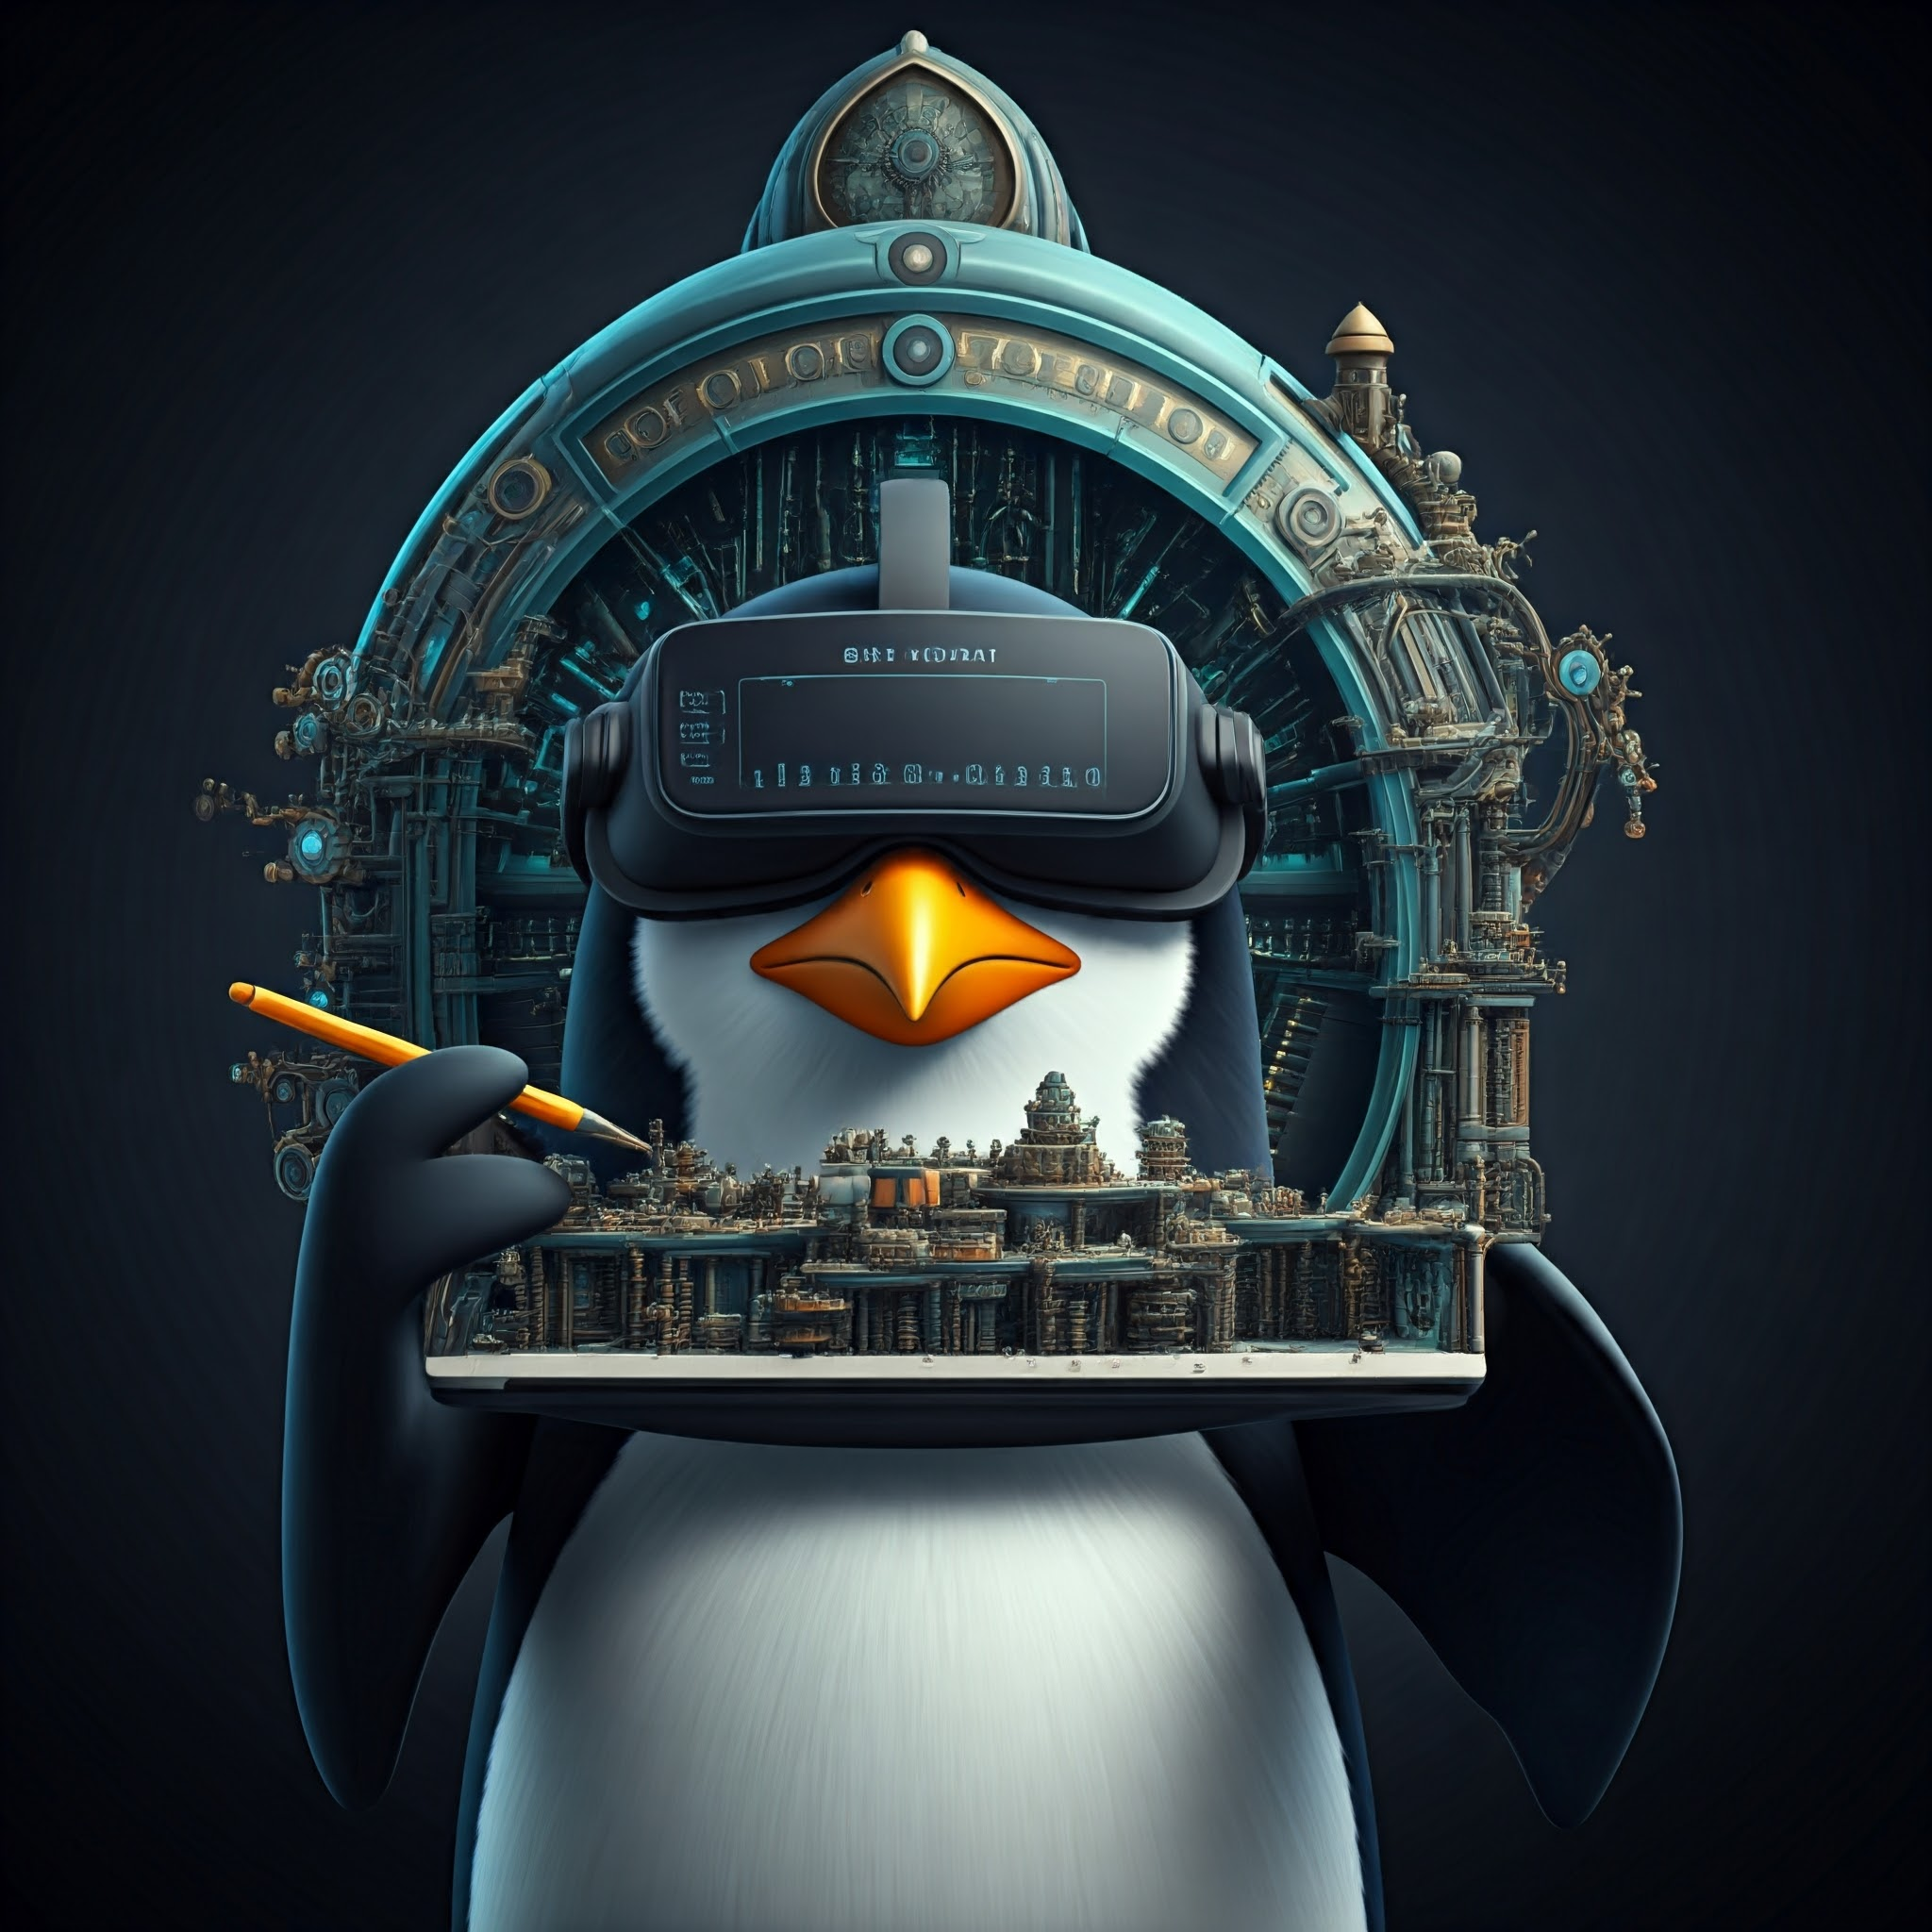
\includegraphics[width=1\textwidth ]{images/Copertina.jpg}
    }
\end{figure}
\vfill 
\centering 
\includegraphics[width=0.4\textwidth ]{../../../preamble/Stemma_sapienza.png} \acc
\centering \Large \color{sapienza}Facoltà di Ingegneria dell'Informazione,
Informatica e Statistica\\
Dipartimento di Informatica
\end{titlepage}

%===================FINE COPERTINA======================%
\newpage
\pagecolor{cartaRiciclata}%\setmainfont{Algerian}
\Large
Questo documento è distribuito sotto la licenza 
\color{blue}\href{https://www.gnu.org/licenses/fdl-1.3.txt}{GNU}\color{black},  
è un resoconto degli appunti (eventualmente integrati con libri di testo) tratti dalle lezioni del corso di Ingegneria del Software
\hphantom{a}per la laurea 
triennale in Informatica. Se dovessi notare errori, ti prego di segnalarmeli.
\vfill
\begin{figure}[h!]
    \raggedright
    
\includegraphics[width=0.4\textwidth,right ]{../../../preamble/tomodachi.pdf} 
\end{figure}
\newpage %\setmainfont{Times New Roman}
\normalsize
\tableofcontents 
\newpage

%==================FOOTER e HEADER=======================%
\fancyhf{}
\fancyhead[L]{\nouppercase{\leftmark}}
\fancyhead[R]{Sezione \thesection}
\fancyfoot[C]{\thepage}
\fancyfoot[L]{Appunti di Ingegneria del Software}
\fancyfoot[R]{ Marco Casu}
%\fancyfoot[R]{\setmainfont{Palace Script MT}\huge Marco Casu \setmainfont{Times New Roman}}
%==================FOOTER e HEADER=======================%

%Ricorda del comando \flowerLine per separare le sottosezioni. Le sezioni si separano nelle diverse pagine

%==================INIZIO======================%
\chapter{Introduzione}
Quando si vuole produrre software complesso, non terminante e di grandi dimensioni, è 
necessario ingegnerizzare il metodo di sviluppo ed astrarre il modello del software. 
L'obiettivo dell'ingegneria del software non riguarda il codice stesso, ma la definizione 
dell'architettura e delle specifiche del sistema. Vanno definiti i processi di sviluppo.\acc 
È cruciale l'analisi dei requisiti, e la modellizazzione delle specifiche di sistema, UML è un 
linguaggio che permette di descrivere la \textit{dinamica} ed il comportamento del modello. Una volta 
definiti i requisiti, si affronta la fase di \textit{planning}.\acc 
Un modello computazionale che risulterà utile prende il nome di \textit{digital twin}, ossia 
una copia del software sulla quale è possibile testare i vari \textit{scenari operativi}, tramite la 
generazione di test automatici. Essendo il sistema discreto, a stati non necessariamente 
finiti, è possibile descriverlo tramite una catena di Markov. \acc 
Nella produzione software prendono parte 3 principali attori\begin{center}
    \includegraphics[width=0.4\textwidth ]{images/attori.eps}
\end{center}
\section{Modellazione}
Il linguaggio UML è utilizzato per modellare sia i requisiti che il sistema stesso, 
esso è composto da differenti diagrammi\begin{itemize}
    \item activity 
    \item use case 
    \item sequence 
    \item class 
    \item state 
    \item context
\end{itemize}
Si consideri il seguente esempio di un sistema di gestione di una clinica psichiatrica, 
lo schema in figura \ref{clinica}, è il context diagram, e rappresenta l'insieme dei serivizi che il 
sistema offre.
\begin{figure}[h!]
    \centering 
    \includegraphics[width=0.7\textwidth ]{images/context.eps}
    \caption{context diagram}
    \label{clinica}
\end{figure}
Un activity diagram descrive l'evoluzione di una certa attività/task che il sistema 
deve poter implementare, si considere l'esempio in figura \ref{activity} riguardante 
l'inserimento di un paziente nella clinica.
\begin{figure}[h!]
    \centering 
    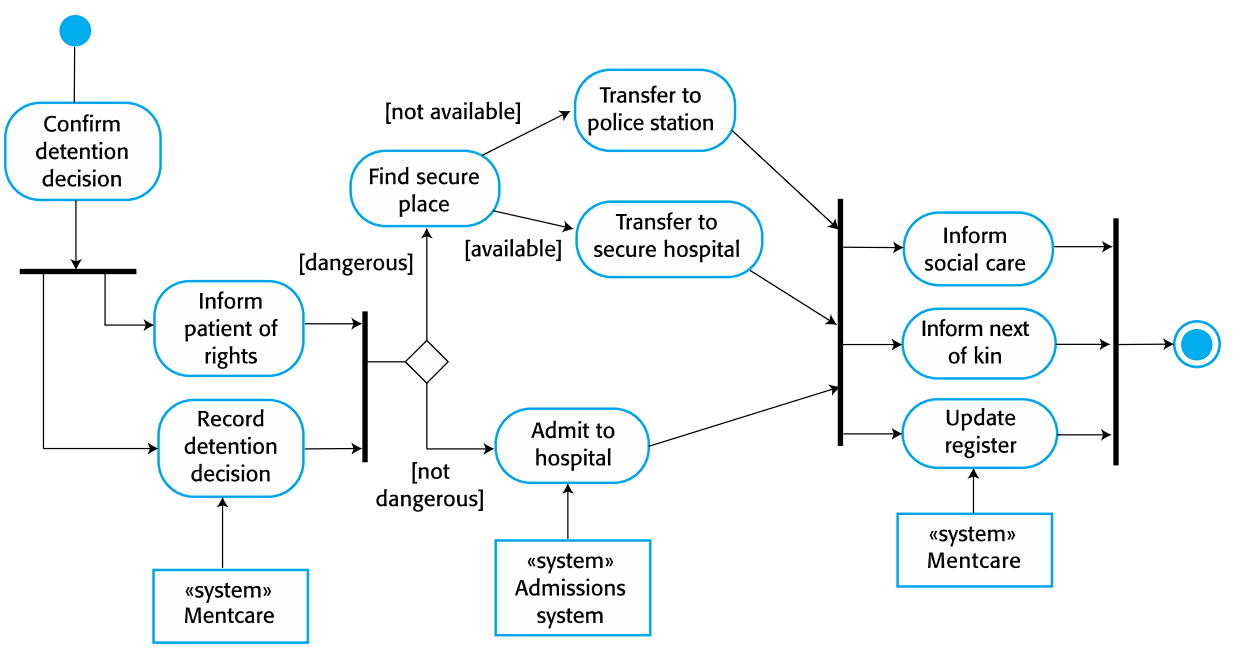
\includegraphics[width=0.7\textwidth ]{images/acrivity.png}
    \caption{activity diagram}
    \label{activity}
\end{figure}
\flowerLine 
\section{Catene di Markov per la Progettazione}
La moderna progettazione di sistemi complessi si basa sul concetto di digital twin, in modo da poter  
definire un modello che simula il sistema su cui verranno eseguiti determinati esperimenti al fine 
di collaudo prima della progettazione vera e propria. Questo capitolo si concetra sull'aspetto \textit{predittivo} 
dei digital twin : Si vuole utilizzare il modello per fare predizioni sull'andamento della 
progettazione.\acc
\defi{(DTMC)} Una \textbf{Catena di Markov Discreta} è una tupla $(U,X,Y,p,g)$ tale che \begin{itemize}
    \item $U$ è un insieme (possibilmente vuoto, finito o non) denotato \textit{input/ingresso} del sistema.
    \item $X$ è un insieme non vuoto  (finito o non) denotato \textit{stato} del sistema.
    \item $Y$ è un insieme non vuoto (finito o non) denotato \textit{output/uscita} del sistema.
    \item $p$ è la \textit{probabilità di transizione}, è una funzione $$p:X\times X\times U\rightarrow[0,1]$$
    tale che $p(x'|x,u)$ rappresenta la probabilità che la DTMC si sposti dallo stato $x$ allo 
    stato $x'$ quando l'ingresso è $u$. Inoltre, per ogni $\tilde x\in X$ e per ogni $\tilde u\in U$, 
    si ha che $$ \int_{x'\in X}p(x'|\tilde x,\tilde u)=1$$
    informalmente, per ogni possibile coppia stato-ingresso, esiste uno stato successivo. 
    \item $g$ è una funzione $$g:X\rightarrow Y$$ detta \textit{funzione di output}.
\end{itemize}
Data una catena di markov $M$, denotiamo $M(U), M(X), M(Y)$ rispettivamente : gli ingressi, gli stati 
e le uscite.\acc 
\textbf{Esempio tempi di completamento} : Si consideri il processo di sviluppo mostrato in figura \ref{esempioDTMC}, si vuole 
calcolare la probabilità che il processo termini in esattamente 10 mesi.\acc 
Si identificano i possibili cammini la cui somma dei sotto processi impiega 10 mesi 
$$ \begin{matrix}
    0\rightarrow 1 \rightarrow  1 \rightarrow2\rightarrow3\rightarrow4 \\
    0\rightarrow 1  \rightarrow2\rightarrow3\rightarrow3\rightarrow4 \\ 
\end{matrix}$$
La probabilità che ciò accada è la somma delle probabilità sui due percorsi 
$$ \begin{matrix}
    1\cdot 0.3 \cdot 0.7 \cdot 0.6 \cdot 0.6 = 0.0756 \\ 
    1\cdot  0.7 \cdot0.6 \cdot0.1 \cdot0.6 = 0.02520
\end{matrix} \implies p(\text{finire in 10 mesi})=0.1008$$
\begin{figure}[h!]
    \centering 
    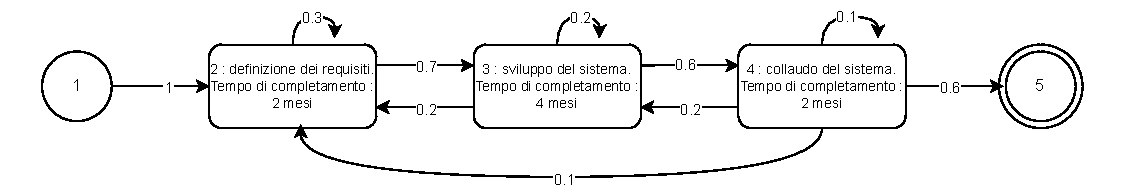
\includegraphics[width=1\textwidth ]{images/esempioDTMC.pdf}
    \caption{Esempio 1}
    \label{esempioDTMC}
\end{figure}\acc 
Qual'è invece la probabilità di finire il processo in esattamente 12 mesi? Si identificano i cammini 
$$ \begin{matrix}
    0\rightarrow1\rightarrow1\rightarrow1\rightarrow2\rightarrow3\rightarrow4\\ 
    0\rightarrow1\rightarrow1\rightarrow2\rightarrow3\rightarrow3\rightarrow4 \\ 
    0\rightarrow1\rightarrow2\rightarrow2\rightarrow3\rightarrow4\\ 
    0\rightarrow1\rightarrow2\rightarrow3\rightarrow3\rightarrow3\rightarrow4
\end{matrix}$$
la probabilità è 
$$\begin{matrix} 1 \cdot 0.3 \cdot 0.3 \cdot 0.7 \cdot 0.6 \cdot 0.6 
    + \\1 \cdot 0.3 \cdot 0.7 \cdot 0.6 \cdot 0.1 \cdot 0.6 +\\
1 \cdot 0.7 \cdot 0.2 \cdot 0.6 \cdot 0.6 + \\
1 \cdot 0.7 \cdot 0.6 \cdot 0.1 \cdot 0.1 \cdot 0.6 =\\
0.022680 + 0.007560 \cdot 0.05040 \cdot 0.002520 =
0.08316\end{matrix}$$
\textbf{Esempio costi di completamento} : Si consideri il processo di sviluppo mostrato in figura \ref{esempioDTMC2}, si vuole 
calcolare la probabilità che il processo abbia un costo toale di esattamente 80.000 euro.\begin{figure}[h!]
    \centering 
    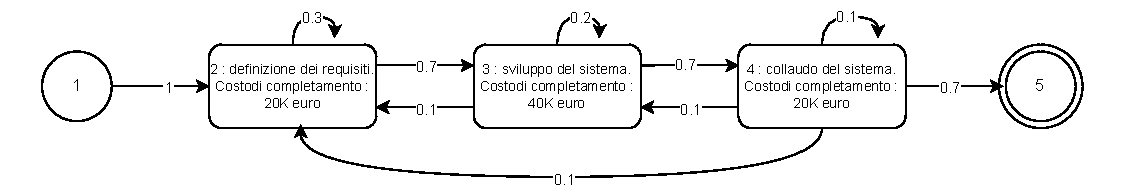
\includegraphics[width=1\textwidth ]{images/esempioDTMC2.pdf}
    \caption{Esempio 2}
    \label{esempioDTMC2}
\end{figure}\acc 
L'unico cammino possibile è$$ \begin{matrix}
    0\rightarrow1\rightarrow2\rightarrow3\rightarrow4
\end{matrix}$$ 
La probabilità è 
$$ 1\cdot 0.7\cdot 0.7 \cdot 0.7 = 0.343$$
\textbf{Esempio costi di design} : Si consideri il processo di sviluppo 
mostrato in figura \ref{esempioDTMC3}, quale deve essere il minimo valore di $p$ tale che 
la probabilità che il processo termini in esattamente 8 mesi sia almeno 0.5?\begin{figure}[h!]
    \centering 
    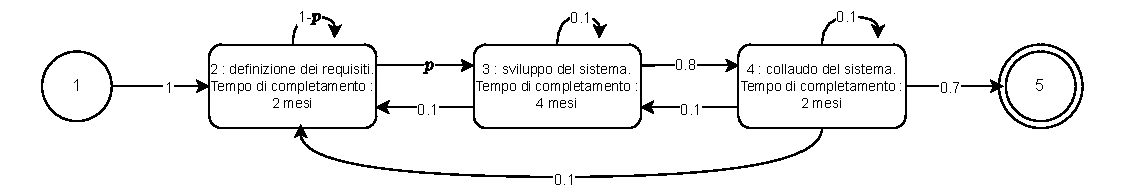
\includegraphics[width=1\textwidth ]{images/esempioDTMC3.pdf}
    \caption{Esempio 3}
    \label{esempioDTMC3}
\end{figure}\acc
L'unico cammino possibile è $$ \begin{matrix}
    0\rightarrow1\rightarrow2\rightarrow3\rightarrow4
\end{matrix}$$ 
la cui probabilità deve essere
$$ 1\cdot p\cdot 0.8 \cdot 0.7 \ge 0.5\implies $$
$$ p\ge \frac{0.5}{0.8\cdot 0.7}=0.8928$$
Una \textbf{rete di catene di Markov} è un insieme di catene di Markov interconnesse 
tramite gli ingressi e le uscite.\begin{center}
    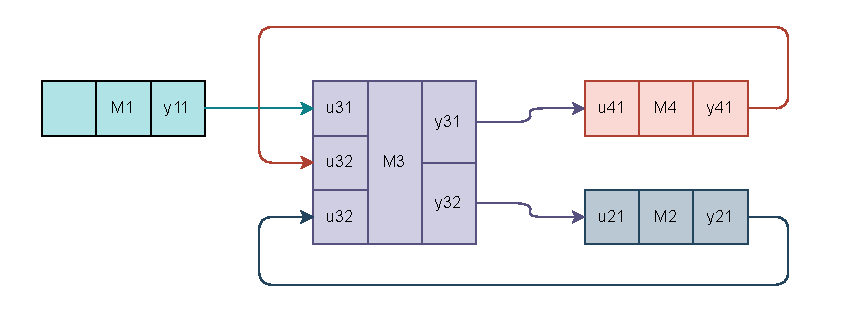
\includegraphics[width=0.8\textwidth ]{images/cateneInterconnesse.pdf}
\end{center}
Inoltre, una rete di catene di Markov è rappresentabile come 
una catena di Markov singola, si considerino le catene di Markov $K,P$ in figura 
\ref{cateneInterconnesse}, formalmente
$$ \begin{matrix}
    K=(U_1\times V, X_1,Y_1,p_1,g_1)\\ 
    P=(U_2, X_2,W\times Z,p_2,(g_{2_w},g_{2_z}))
\end{matrix}$$
\begin{figure}[h!]
    \centering 
    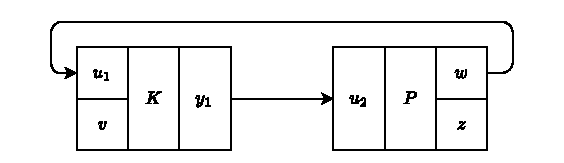
\includegraphics[width=0.7\textwidth ]{images/cateneInterconnesse2.pdf}
    \caption{$K$ e $P$ interconnesse}
    \label{cateneInterconnesse}
\end{figure}\acc
Nota : $u_1$ rappresenta un elemento dell'insieme $U_1$ (ingresso di $K$), $v\in V$, $y_1\in Y_1\dots$ analogo 
per gli altri elementi.\acc
Un ingresso di $K$ è un uscita di $P$ $$ M_1(U_1)=M_2(W)$$ 
e l'ingresso di $P$ è l'uscita di $K$ $$ M_2(U_2)=M_1(Y_1)$$
Si può definire il sistema globale equivalente 
$$M=(V,X_1\times X_2,Z,p,g) $$
Dove \begin{itemize}
    \item $p((x_1',x_2')|(x_1,x_2),v)=p_1(x_1'|x_1,(g_{2_w}(x_2),v))\cdot p_2(x_2'|x_2,g_1(x_1))$ 
    \item $g(x_1,x_2)=g_{2_z}(x_2)$\begin{center}
        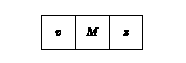
\includegraphics[width=0.4\textwidth ]{images/vmz.pdf}
    \end{center}
\end{itemize}\flowerLine 
\section{Implementazione delle DTMC}
In questa sezione verrà trattata una possibile implementazione delle DTMC in \textit{C++}. Si assume che il lettore sia a conoscenza delle regole di scrittura e strutturazione degli header e file C. \acc 
Una DTMC sarà implementata in due file \\
\shell{dtmc.h}\\ 
\shell{dtmc.cpp}\\
Nel file \code{dtmc.h} come prima cosa, si definisce il \textit{tipo} delle variabili di ingresso, stato, e 
uscita, tramite il costrutto \code{typedef}.\begin{lstlisting}[style=CppStyle,language=C++]
typedef double state_type;
typedef double input_type;
typedef double output_type;
\end{lstlisting}
Va poi definita la classe \code{DTMC} le cui istanze rappresenteranno proprio le catene di Markov, gli elementi privati di tale classe saranno 2\begin{itemize} 
    \item Un puntatore ad una classe \code{RandGen} definita in un'apposito file \code{randgen.cpp}
    \item Una funzione \code{dtmc\_body} che verrà definita nel file \code{dtmc.cpp}
\end{itemize}
\begin{lstlisting}[style=CppStyle,language=C++]
class DTMC {

private:
    RandGen *p;  // pointer to random generator class 
    void dtmc_body(RandGen *p);
\end{lstlisting}
Fra gli elementi pubblici della classe ci saranno poi le dimensioni dei vettori di ingresso, stato ed uscita [di default, assumeremo che tali vettori siano in $\R^2$], insieme a delle variabili che rappresentano lo stato corrente, l'ingresso e l'uscita. Ci saranno poi due costruttori, uno più esplicito dell'altro\begin{itemize}
    \item Il primo costruttore riceve in ingresso esclusivamente il puntatore all'oggetto di tipo 
    \code{RandGen}, lasciando invariate le dimensioni dei vettori di stato, ingresso ed uscita a 2. 
    \item Il secondo costruttore è più esplicito e permette la modifica delle dimensioni dei vettori di stato, ingresso ed uscita.
\end{itemize}
\begin{lstlisting}[style=CppStyle,language=C++]
public:
    int STATE_SIZE = 2; // state size
    int INPUT_SIZE = 2; // input size
    int OUTPUT_SIZE = 2; // output size
  
    state_type *x;  // present state
    input_type *u;  // input
    output_type *y;  // output
  
    DTMC(RandGen *p);
    DTMC(int xsize, int usize, int ysize, RandGen *p);  
\end{lstlisting}
Ci sono poi le varie funzioni della classe, precisamente per \begin{itemize}
    \item inizializzare la catena con lo stato iniziale 
    \item calcolare il prossimo stato dato lo stato attuale e l'ingresso 
    \item dato uno stato restituisce l'uscita del sistema
\end{itemize}
Ci sono poi due funzioni di servizio per la visualizzazione dello stato in console (oppure su un file).
\begin{lstlisting}[style=CppStyle,language=C++]
    // define initial state
    void init();
  
    // update state
    void next();
    
    // update output
    void output();
  
    // print log on stdout
    void printlog(int t);
  
    // print log on file
    void fprintflog(FILE *fp, int t);
\end{lstlisting}
Verrà considerata adesso la definizione delle funzioni dichiarate, precisamente, nel file \code{dtmc.cpp}. Ovviamente vanno incluse le dichiarazioni.
\begin{lstlisting}[style=CppStyle,language=C++]
#include "dtmc.h"
using namespace std;
\end{lstlisting}
La funzione \code{dtmc\_body} verrà richiamata dai costruttori per definire ed inizializzare la catena di Markov. Deve ricevere in input il puntatore al generatore di numeri casuali ed assegnarlo alla variabile interna (privata). Dopo aver fatto ciò 
viene fatto un controllo sulle dimensioni del vettore di stato che devono essere strettamente 
maggiori di zero.
\begin{lstlisting}[style=CppStyle,language=C++]
void dtmc_body(RandGen *myp) {
    p = myp;
    if (STATE_SIZE <= 0)
    {
     fprintf(stderr, "DTMC(): Error: state size cannot be 0\n");
     exit(1);
    }
\end{lstlisting}
A questo punto, bisogna inizializzare il vettore di stato, dato che le dimensioni non sono note 
a priori, sarà necessario allocare dinamicamente lo spazio. 
\begin{lstlisting}[style=CppStyle,language=C++]
    x = (state_type *) malloc(sizeof(state_type)*STATE_SIZE);

    if (x == NULL)
        {
        fprintf(stderr, "DTMC(): memory allocation for state failed\n");
        exit(1);
    }
\end{lstlisting}
Si prosegue analogamente con l'ingresso e l'uscita, si ricordi che una DTMC può avere ingresso nullo, ma deve necessariamente esserci un uscita.
\begin{lstlisting}[style=CppStyle,language=C++]
    if (INPUT_SIZE <= 0)
    {
        u = NULL;
    }
    else
    {
        u = (input_type *) malloc(sizeof(input_type)*INPUT_SIZE);
        if (u == NULL)
        {
            fprintf(stderr, "DTMC(): memory allocation 
                                for input failed\n");
            exit(1);
        }
    }
    
    if (OUTPUT_SIZE <= 0)
    {
        fprintf(stderr, "DTMC(): Error: output size cannot be 0\n");
        exit(1);
    }

    y = (output_type *) malloc(sizeof(output_type)*OUTPUT_SIZE);
    if (y == NULL)
    {
        fprintf(stderr, "DTMC(): memory allocation 
                            for output failed\n");
        exit(1);
    }
}
\end{lstlisting}
A tal punto i due costruttori possono richiamare tale funzione per inizializzare la catena.
\begin{lstlisting}[style=CppStyle,language=C++]
DTMC(RandGen *myp)  {
    dtmc_body(myp);
}
          
DTMC(int xsize, int usize, int ysize, RandGen *myp)  {    
    STATE_SIZE = xsize;
    INPUT_SIZE = usize;
    OUTPUT_SIZE = ysize;
    dtmc_body(myp);
}
\end{lstlisting}
La funzione di inizializzazione inizializza a zero il vettore di stato.
\begin{lstlisting}[style=CppStyle,language=C++]
void init() {
    /* initial state */
    for (int i = 0; i < STATE_SIZE; i++)
    {
        x[i] = 0;
    }
}
\end{lstlisting}
La funzione \code{next} dovrà calcolare lo stato successivo
\begin{lstlisting}[style=CppStyle,language=C++]
void next() {
    /* initial state */
    for (int i = 0; i < STATE_SIZE; i++)
    {
        x[i] = p -> get_random_double();
    }
}
\end{lstlisting}
La funzione \code{get\_random\_double} è definita in \code{RandGen} e restituisce un double casuale compreso fra 0 e 1. In questo caso specifico, lo stato è un vettore di numeri reali, quindi è una DTMC a stati infiniti. Si definisce poi la funzione in output, in questo specifico caso, l'output sarà identico allo stato.
\begin{lstlisting}[style=CppStyle,language=C++]
void output() {
    /* initial state */
    for (int i = 0; i < OUTPUT_SIZE; i++)
    {
        y[i] = x[i];
    }
}
\end{lstlisting}
Ovviamente le dimensioni devono combaciare. Si definiscono poi le funzioni di servizio che 
si occuperanno di eseguire un print dello stato della catena di Markov in formato CSV, così poi 
da rendere facile la generazione di un grafico.
\begin{lstlisting}[style=CppStyle,language=C++]
void printlog(int t) {
    /* t e' il tempo corrente */
    int i;
    printf("%d ", t);
    for (i = 0; i < STATE_SIZE; i++)
    {
        printf("%lf ", x[i]);
    }
    for (i = 0; i < OUTPUT_SIZE; i++)
    {
        printf("%lf ", y[i]);
    }
    for (i = 0; i < INPUT_SIZE; i++)
    {
        printf("%lf ", u[i]);
    }
    printf("\n");
} 
\end{lstlisting}
La funzione \code{fprintflog} è analoga ma scrive su un file.\acc 
Si da ora una descrizione della classe \code{RandGen}, definita nei file\\
\shell{randgen.h}\\ 
\shell{randgen.cpp}\\
Il file header è molto semplice, contiene la dichiarazione del costruttore, una variabile (seed) e due funzioni per la generazione di numeri double e interi.
\begin{lstlisting}[style=CppStyle,language=C++]
class RandGen{
public:
    RandGen();
    unsigned int seed;
    double get_random_double();
    int get_random_int();
}
\end{lstlisting}
Il seed è un intero che condiziona la generazione dei valori. Il file \code{randgen.cpp} contiene ovviamente le definizioni ed utilizza una serie di funzioni già preesistenti del C++ definite nella libreria matematica. Oltre ad includere il file header, si utilizza un oggetto già definito per la generazione del seed. Dopo di ciò, si inizializzano arbitrariamente delle distribuzioni. Nell'esempio 
seguente, per i double i valori che possono essere estratti sono compresi fra 0 ed 1, per gli interi da -10 a 10.
\begin{lstlisting}[style=CppStyle,language=C++]
#include "randgen.h"
random_device myRandomDevice;
unsigned int myseed = myRandomDevice();

default_random_engine myRandomEngine(myseed);
uniform_int_distribution<int> myUnifIntDist(-10,10);
uniform_real_distribution<double> myUnifRealDist(0.0,1.0);
RandGen(){
    seed=myseed;
}
\end{lstlisting}
Si definiscono poi le funzioni che generano il numero casuale.
\begin{lstlisting}[style=CppStyle,language=C++]
double get_random_double() {
  return(myUnifRealDist(myRandomEngine));
} 

int RandGen::get_random_int() {
  return(myUnifIntDist(myRandomEngine));
} 
\end{lstlisting}
A questo punto, si è definita in tutto e per tutto una catena di markov a tempo discreto, si vuole scrivere un \textit{simulatore} che si occupi di istanziare la classe e di eseguire dei test. Si definiscono quindi due file\\
\shell{simulator.h}\\ 
\shell{simulator.cpp}\\
Come prima cosa nel file header si definisce la classe \code{Simulator} i cui oggetti faranno "muovere" la/le catena/e di Markov. È una classe con una sola funzione pubblica.
\begin{lstlisting}[style=CppStyle,language=C++]
#include "main.h"
class Simulator {
public:
  // run simulation with horizon T
  void run(int T);
};
\end{lstlisting}
La funzione \code{run} prende come argomento "l'orizzonte", ossia il numero di step finiti che la catena di Markov deve compiere.\acc  Il simulatore è in tutto e per tutto la funzione \code{run} definita nel file \code{simulator.cpp}, che definisce come prima cosa gli elementi necessari alla DTMC.
\begin{lstlisting}[style=CppStyle,language=C++]
void Simulator(int T){
    RandGen p; 
    DTMC mc1(&p);
    int t=0;
    FILE *fp;
    printf("seed : %u\n",p.seed); //servizio
    printf("inizialization : t=  %d\n",t); //servizio
    mc1.init();
    fp=fopen("logfile.csv","w");
\end{lstlisting}
Il tempo \code{t} si inizializza a zero. Il file \code{fp} sarà quello in cui verrà scritto il log della catena. A tal punto va eseguita la simulazione vera e propria eseguendo precisamente \code{T} step sulla catena di Markov, scrivendo lo stato sul log ad ogni passo.
\begin{lstlisting}[style=CppStyle,language=C++]
    for (t = 0; t <= T; t++)
    {
        mc1.output();
        mc1.u[0] = t;  mc1.u[1] = mc1.y[1] + 1;
        mc1.printlog(t);
        mc1.fprintflog(fp, t);
        mc1.next(); 
        #if 0
            printf("get state of system at time %d\n", t);
            printf("get output of system at time %d\n", t);
            printf("update inputs with outputs at time %d\n", t);
            printf("update state of system with
                    inputs at time %d\n\n", t);
        #endif  
    }  
    fclose(fp);
    }  
\end{lstlisting}
Ad ogni passo, il vettore in input assume il valore (tempo,uscita + 1). L'output si ricordi essere funzione esclusivamente dello stato e non dell'input, è quindi perfettamente legittimo utilizzare come input l'uscita del sistema, in tal modo detto "a retroazione".
$$ u(t)=\begin{bmatrix}
    t \\ 
    y(t-1)+1
\end{bmatrix}$$
Il progetto può essere poi compilato con un makefile, un possibile makefile generico è il seguente.
\begin{lstlisting}[language=make]
CC=g++
#CFLAGS=-std=c++11 -lm -I. -I/usr/include/postgresql -lpq 
#CFLAGS=-std=c++11 -I. -I/usr/include/postgresql -lpq -lm 
CFLAGS=-std=c++11 -I.  -lm 
DEPS = $(wildcard *.h)
objects := $(patsubst %.cpp,%.o,$(wildcard *.cpp))
%.o:	%.cpp $(DEPS)
    $(CC) -c -o $@ $< $(CFLAGS)

main: 	$(objects)
    $(CC) -o main $(objects) $(CFLAGS)
clear:
    rm *.o 
clearall:
    rm main ; rm *.o 
\end{lstlisting}
%FILE CODICE
\newpage 
\section{Raccolta dei File}
\subsection{\code{main.h}}
\begin{lstlisting}[style=CppStyle,language=C++]
#ifndef main_h
#define main_h
    
using namespace std;
    
#include <iostream>
#include <random>
    
#include "randgen.h"
#include "dtmc.h"
#include "simulator.h"
    
#if 0
#include "clock.h"
#include "logger.h"
#include "gtime.h"
#include "timer.h"
#include "basic.h"
#include "system.h"
    
#include "ctr.h"
#include "plant.h"
#include "root.h"
#endif
     
#define DEBUG 1000
    
#define HORIZON 10
    
#if 0
extern Logger val2log;
extern GlobalTime gtime;
extern Clock ck;
extern random_device myRandomDevice;
extern unsigned int seed;
extern default_random_engine myRandomEngine;
extern uniform_int_distribution<int> myUnifIntDist;
extern uniform_real_distribution<double> myUnifRealDist;
#endif
    
#if 0
    random_device myRandomDevice;
    unsigned int seed = myRandomDevice();  
// Initialize a default_random_engine with the seed
    default_random_engine myRandomEngine(seed);
// Initialize a uniform_int_distribution to produce values between -10 and 10
    uniform_int_distribution<int> myUnifIntDist(-10, 10);
// Initialize a uniform_real_distribution to produce values between 0 and 1
    uniform_real_distribution<double> myUnifRealDist(0.0, 1.0);
#endif 
#endif
\end{lstlisting}

\newpage 
\subsection{\code{dtmc.h}}
\begin{lstlisting}[style=CppStyle,language=C++]
#ifndef dtmc_h
#define dtmc_h
    
#include "main.h" /*include il file dove e'
                     definita la classe RandGen*/
    
typedef double state_type;
typedef double input_type;
typedef double output_type;
    
class DTMC {
    
private:
    
    RandGen *p;  // pointer to random generator class
      
    void dtmc_body(RandGen *p);
    
public:
    
    int STATE_SIZE = 2; // state size
    int INPUT_SIZE = 2; // input size
    int OUTPUT_SIZE = 2; // output size
    
    state_type *x;  // present state
    input_type *u;  // input
    output_type *y;  // output
    
    DTMC(RandGen *p);
    DTMC(int xsize, int usize, int ysize, RandGen *p);
    
    // define initial state
    void init();
    
    // update state
    void next();
      
    // update output
    void output();
    
    // print log on stdout
    void printlog(int t);
    
    // print log on file
    void fprintflog(FILE *fp, int t);
};
    
#endif
\end{lstlisting}


\newpage 
\subsection{\code{dtmc.cpp}}
\begin{lstlisting}[style=CppStyle,language=C++]
#include "main.h"
#include "dtmc.h"

void dtmc_body(RandGen *myp) {
    p = myp;
    if (STATE_SIZE <= 0)
    {
        fprintf(stderr, "DTMC(): Error: state size cannot be 0\n");
        exit(1);
    } 
    x = (state_type *) malloc(sizeof(state_type)*STATE_SIZE);
    if (x == NULL)
    {
        fprintf(stderr, "DTMC(): memory allocation for state failed\n");
        exit(1);
    }
    if (INPUT_SIZE <= 0)
    {
        u = NULL;
    }
    else
    {
        u = (input_type *) malloc(sizeof(input_type)*INPUT_SIZE);
        if (u == NULL)
        {
            fprintf(stderr, "DTMC(): memory allocation 
                             for input failed\n");
            exit(1);
        }
    } 
    if (OUTPUT_SIZE <= 0)
    {
        fprintf(stderr, "DTMC(): Error: output size cannot be 0\n");
        exit(1);
    }
    y = (output_type *) malloc(sizeof(output_type)*OUTPUT_SIZE);
    if (y == NULL)
    {
        fprintf(stderr, "DTMC(): memory allocation 
                         for output failed\n");
        exit(1);
    } 
}


DTMC(RandGen *myp)  {
    dtmc_body(myp);
}

DTMC(int xsize, int usize, int ysize, RandGen *myp)  {
    STATE_SIZE = xsize;
    INPUT_SIZE = usize;
    OUTPUT_SIZE = ysize;
    dtmc_body(myp);  
}

void init() {
    int i;
    for (i = 0; i < STATE_SIZE; i++)
        x[i] = 0;
}  
void next() {
    int i;
    for (i = 0; i < STATE_SIZE; i++)
        x[i] = p -> get_random_double();
}
void output() {
    int i;
    for (i = 0; i < OUTPUT_SIZE; i++)
        y[i] = x[i];
}

void printlog(int t) {
    int i;
    printf("%d ", t);
    for (i = 0; i < STATE_SIZE; i++)
    {
        printf("%lf ", x[i]);
    }
    for (i = 0; i < OUTPUT_SIZE; i++)
    {
        printf("%lf ", y[i]);
    }
    for (i = 0; i < INPUT_SIZE; i++)
    {
        printf("%lf ", u[i]);
    }
    printf("\n");
} 

void fprintflog(FILE *fp, int t) {
    FILE *fp;
    int i;
    fp = fopen(filename, "w");
    fprintf(fp, "%d ", t);
    for (i = 0; i < STATE_SIZE; i++)
    {
        fprintf(fp, "%lf ", x[i]);
    }
    for (i = 0; i < OUTPUT_SIZE; i++)
    {
        fprintf(fp, "%lf ", y[i]);
    }
    for (i = 0; i < INPUT_SIZE; i++)
    {
        fprintf(fp, "%lf ", u[i]);
    }
    fprintf(fp, "\n");
}
\end{lstlisting} 


\newpage 
\subsection{\code{randgen.h}}
\begin{lstlisting}[style=CppStyle,language=C++]
#ifndef randgen_h
#define randgen_h
#include "main.h"

class RandGen {
public:
    RandGen();
    unsigned int seed;
    double get_random_double();
    int get_random_int(); 
};
#endif
\end{lstlisting} 
\subsection{\code{randgen.cpp}}
\begin{lstlisting}[style=CppStyle,language=C++]
#include "main.h"
#include "randgen.h"

random_device myRandomDevice;
unsigned int myseed = myRandomDevice();

default_random_engine myRandomEngine(myseed);
uniform_int_distribution<int> myUnifIntDist(-10, 10);
uniform_real_distribution<double> myUnifRealDist(0.0, 1.0);
RandGen() { seed = myseed; }

double get_random_double() {
    return(myUnifRealDist(myRandomEngine));
} 

int get_random_int() {
    return(myUnifIntDist(myRandomEngine)); 
} 
\end{lstlisting} 
%FINE FILE CODICE








\chapter{Planning del Progetto}
Il planning di un progetto, consiste nel suddividere il carico di lavoro in diverse 
parti, da assegnare ai vari membri del team, cercando di prevedere possibili problemi 
che potrebbero insorgere durante lo sviluppo, pensando e preparando eventuali modi per 
risolverli.\acc 
Il \textit{piano del progetto} viene preparato all'inizio dei lavori, viene utilizzato per 
comunicare ai vari membri del team ed al cliente come esso è stato suddiviso. Le fasi in cui 
il planning viene definito sono \begin{itemize}
    \item Durante la proposta, quando avviene la contrattazione con il cliente riguardo lo sviluppo del 
    software 
    \item Durante la fase di avvio dei lavori, quando si decide come e a chi assegnare il lavoro, e 
    quali risorse dovranno essere allocate 
    \item Periodicamente durante lo sviluppo, monitorando ed appositamente modificando i piani in base 
    all'andamento del progetto e alle esperienze pregresse
\end{itemize}
Lo scopo del planning è quello di avere un idea chiara sul progetto in modo che si possa decidere 
un prezzo d'accordo con il cliente, valutando e stimando quanto denaro sarà necessario per 
lo sviluppo considerando variabili del tipo \begin{itemize}
    \item costo dei dipendenti 
    \item costo dell'hardware necessario 
    \item costo del software
\end{itemize}
Durante la fase di planning, sono noti i requisiti del sistema, ma non è ancora chiara la 
struttura del software, tanto meno la sua implementazione, il planning deve essere 
preciso a sufficienza per far si che sia possibile definire il budget e lo staff necessario. 
Inoltre bisogna definire i meccanismi con la quale verrà monitorato lo sviluppo.
\flowerLine
\section{Sviluppo Plan-Driven}
Con \textit{plan driven development}, si intende un approccio all'ingegneria del software in cui 
i processi di sviluppo sono programmati in principio, in maniera dettagliata. Si basa sulle tecniche di 
gestione, tipiche dei progetti ingegneristici, e sulle tecniche "classiche" di gestione di grandi 
progetti software.\acc 
Un project plan ha l'obiettivo di definire e monitorare il lavoro da svolgere, in che modo 
deve essere svolto, da chi, e quali prodotti sono necessari. È scopo del manager, servirsi di un project 
plan (che da ora chiameremo semplicemente "piano") 
per supportare le decisioni da prendere durante lo sviluppo, e per misurarne il progresso.\begin{itemize}
    \item Un lato favorevole di tale approccio, è che una pianificazione a monte permette di 
    aggirare problemi organizzativi in principio, determinando potenziali problemi e dipendenze 
    da soddisfare prima che il progetto sia avviato, piuttosto che durante la lavorazione. \begin{quote}
        \textit{meglio prevenire che curare}
    \end{quote}
    \item Un lato sfavorevole, è che molte decisioni prese in principio vanno riviste dati possibili 
    cambiamenti dell'ambiente in cui il software deve essere adoperato.
\end{itemize}
Un piano deve definire, le risorse disponibili per il progetto, la suddivisione 
del carico di lavoro, una schedule per portare a termine il lavoro. Precisamente, un piano consiste 
nelle seguenti sezioni\begin{enumerate}
    \item introduzione 
    \item organizzazione del progetto 
    \item analisi dei rischi 
    \item risorse hardware e software necessarie 
    \item struttura di scomposizione del lavoro
    \item schedule del progetto 
    \item meccanismi di monitoraggio e report
\end{enumerate}
Ci sono inoltre altri tipi di "piano" che possono essere aggiunti a quello principale come supporto:
\begin{center}
    \begin{tabular}{cc}
        \rowcolor[HTML]{9698ED} 
        Piano                                           & Descrizione                                                                                                                                                                                                                                                              \\
                                                        &                                                                                                                                                                                                                                                                          \\
        \rowcolor[HTML]{DAE8FC} 
        \textbf{Configuration managment plan}           & \begin{tabular}[c]{@{}c@{}}descrive la configurazione delle \\ procedure di gestione, la loro \\ struttura ed il loro utilizzo\end{tabular}                                                                                                                              \\
        \rowcolor[HTML]{ECF4FF} 
        {\color[HTML]{000000} \textbf{Deployment plan}} & {\color[HTML]{000000} \begin{tabular}[c]{@{}c@{}}descrive come il software deve \\ essere integrato con l'apposito \\ hardware di riferimento del cliente, \\ con eventuali piani di migrazione dei \\ dati in uso su sistemi precedentemente \\ adoperati\end{tabular}} \\
        \rowcolor[HTML]{DAE8FC} 
        \textbf{Maintenance plan}                       & \begin{tabular}[c]{@{}c@{}}predizione dei requisiti, costi e lavoro \\ per la manutenzione del software\end{tabular}                                                                                                                                                     \\
        \rowcolor[HTML]{ECF4FF} 
        {\color[HTML]{000000} \textbf{Quality plan}}    & {\color[HTML]{000000} \begin{tabular}[c]{@{}c@{}}descrizione delle procedure e standard di \\ qualità utilizzati nel progetto\end{tabular}}                                                                                                                              \\
        \rowcolor[HTML]{DAE8FC} 
        \textbf{Validation plan}                        & \begin{tabular}[c]{@{}c@{}}descrizione degli approcci, risorse e schedule \\ utilizzati per la convalida del sistema\end{tabular}                                                                                                                                       
        \end{tabular}
\end{center}
Il planning del progetto è un processo \textit{iterativo} che viene sottoposto 
ad inevitabili cambiamenti durante lo sviluppo progressivo. Con l'aumentare delle informazioni 
relative al sistema durante lo sviluppo, è doveroso revisionare i requisiti iniziali,  
dei cambiamenti nel business possono portare a grandi cambiamenti nei requisiti del progetto, portando 
ad un eventuale ri-pianificazione totale.
\subsubsection{Assuzioni del planning}\begin{itemize}
    \item Le assunzioni da fare durante la definizione del project plan 
    non devono essere ottimistiche, bensì 
    realistiche.
    \item Durante lo sviluppo insorgeranno inevitabilmente dei problemi che causeranno dei ritardi 
    nella consegna. 
    \item Le assunzioni iniziali e lo scheduling saranno inevitabilmente soggetti a problemi inaspettati.
    \item Bisogna sempre considerare ogni imprevisto, in modo che eventuali problemi non 
    siano troppo gravanti sulla schedule.
\end{itemize}\begin{center}
\begin{figure}[h!]
    \centering 
    \includegraphics[width=1\textwidth ]{images/projectPlanning.eps}
    \caption{Processi del project planning}
\end{figure}\end{center}
In caso di seri problemi durante lo sviluppo, è necessario applicare delle procedure di 
\textit{mitigazione del rischio}, onde evitare il fallimento del progetto. In congiunzione a ciò, 
può essere necessaria la ripianificazione del progetto.\\ 
Ciò può comportare la rinegoziazione con il cliente dei risultati attesi 
e dei vincoli da rispettare. Una nuova schedule, e data di consegna dovrà essere definita in modo 
da stabilire un accordo con il cliente.
\flowerLine 
\section{Scheduling del Progetto}
\defi{} : Con \textit{scheduling del progetto} si intende il processo di decisione riguardante 
il come il carico di lavoro di un progetto deve essere organizzato in differenti attività, ed 
in che ordine queste attività devono essere eseguite.\acc 
Viene stimato un calendario con i tempi necessari al completamento delle attività, lo sforzo 
necessario ed il personale al quale delegarlo. È anche necessaria una stima delle risorse 
necessarie, come lo spazio su disco necessario per il software, ed il budget da 
muovere.\begin{enumerate}
    \item Suddivisione del progetto in varie attività e stima delle risorse per ognuna di esse 
    \item Organizzazione delle attività da eseguire in concorrenza per ottimizzare i tempi 
    \item Minimizzazione delle dipendenze fra le varie attività, in modo da ridurre i 
    ritardi dovuti ad attese 
\end{enumerate}
Questi ultimi fattori dipendono anche dall'intuizione e dalla esperienza del project manager.
\begin{center}
    \begin{figure}[h!]
        \centering 
        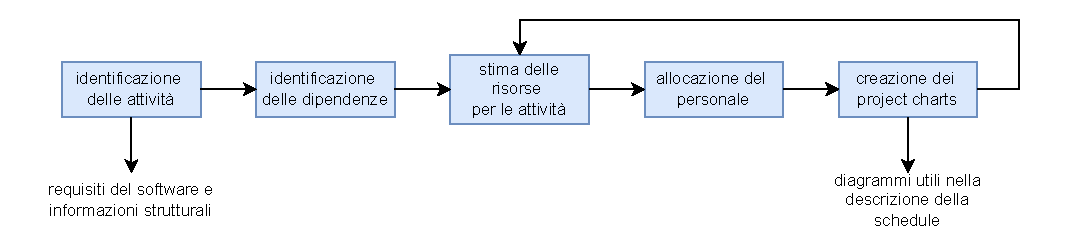
\includegraphics[width=1\textwidth ]{images/projectScheduling.pdf}
        \caption{Scheduling}
    \end{figure}\end{center}
\subsubsection{Problemi nello scheduling}\begin{itemize}
    \item Stimare la difficoltà del lavoro ed i costi di sviluppo è molto difficile 
    \item La produttività non è proporzionale al numero di persone coinvolte nel lavoro 
    \item L'aggiunta di personale a progetto già avviato può causare ritardi  
    \item Accade sempre l'inaspettato, bisogna considerare ogni evenienza nel planning
\end{itemize}
Esiste un annotazione grafica utile nella rappresentazione 
della schedule, mostra le diverse attività, il periodo in cui 
vanno terminate e le varie dipendenze fra esse, il diagramma a barre 
mostra le attività come risorse da disporre sull'asse dei 
tempi. Le "project activities" sono gli elementi di base del 
grafico, comprendono \begin{itemize}
    \item una durata sul calendario, di giorni o mesi 
    \item un carico di lavoro stimato, misurato in numero di 
    impiegati al giorno necessari
    \item una deadline per ogni attività che ne vincola 
    il completamento entro una certa data
    \item un punto specifico che descrive il terminamento di 
    un'attività, può essere un documento , una riunione o il completamento 
    di tutti i test
\end{itemize}
Una \textbf{milestone} non è altro che una "tappa 
fondamentale" durante lo svolgimento delle varie attività, può 
rappresentare un momento in cui si valuta la progressione del 
progetto.\acc 
Con \textbf{deliverables} si definiscono dei risultati ottenuti 
durante la lavorazione da presentare al cliente.
\begin{center}
    \begin{tabular}{|c|c|c|c|}
        \hline
        \rowcolor[HTML]{CBCEFB} 
        task & \begin{tabular}[c]{@{}c@{}}personale necessario \\ (persone/giorno)\end{tabular} & durata in giorni & dipendenze    \\ \hline
        \rowcolor[HTML]{ECF4FF} 
        T1   & 15                                                                               & 10               &               \\ \hline
        T2   & 8                                                                                & 15               &               \\ \hline
        \rowcolor[HTML]{ECF4FF} 
        T3   & 20                                                                               & 15               & T1 (M1)       \\ \hline
        T4   & 5                                                                                & 10               &               \\ \hline
        \rowcolor[HTML]{ECF4FF} 
        T5   & 5                                                                                & 10               & T2,T4 (M3)    \\ \hline
        T6   & 10                                                                               & 5                & T1,T2 (M4)    \\ \hline
        \rowcolor[HTML]{ECF4FF} 
        T7   & 25                                                                               & 20               & T1 (M1)       \\ \hline
        T8   & 75                                                                               & 25               & T4 (M2)       \\ \hline
        \rowcolor[HTML]{ECF4FF} 
        T9   & 10                                                                               &                  & T3,T6 (M5)    \\ \hline
        T10  & 20                                                                               & 15               & T7,T8 (M6)    \\ \hline
        \rowcolor[HTML]{ECF4FF} 
        T11  & 10                                                                               & 10               & T9 (M7)       \\ \hline
        T12  & 20                                                                               & 10               & T10, T11 (M8) \\ \hline
        \end{tabular}
\end{center}
Nella tabella sopramostrata, sono riportate diverse attività di un processo 
di sviluppo, ogni attività $T_i$ (o task) ha associato un certo numero di persone necessarie ed 
una durata in giorni. Inoltre, un task può dipendere da uno o più task. Con $M_i$ si 
identificano le milestones.
\begin{center}
	\begin{tabular}{>{\centering\arraybackslash}m{3in}>{\arraybackslash}m{3in}}
        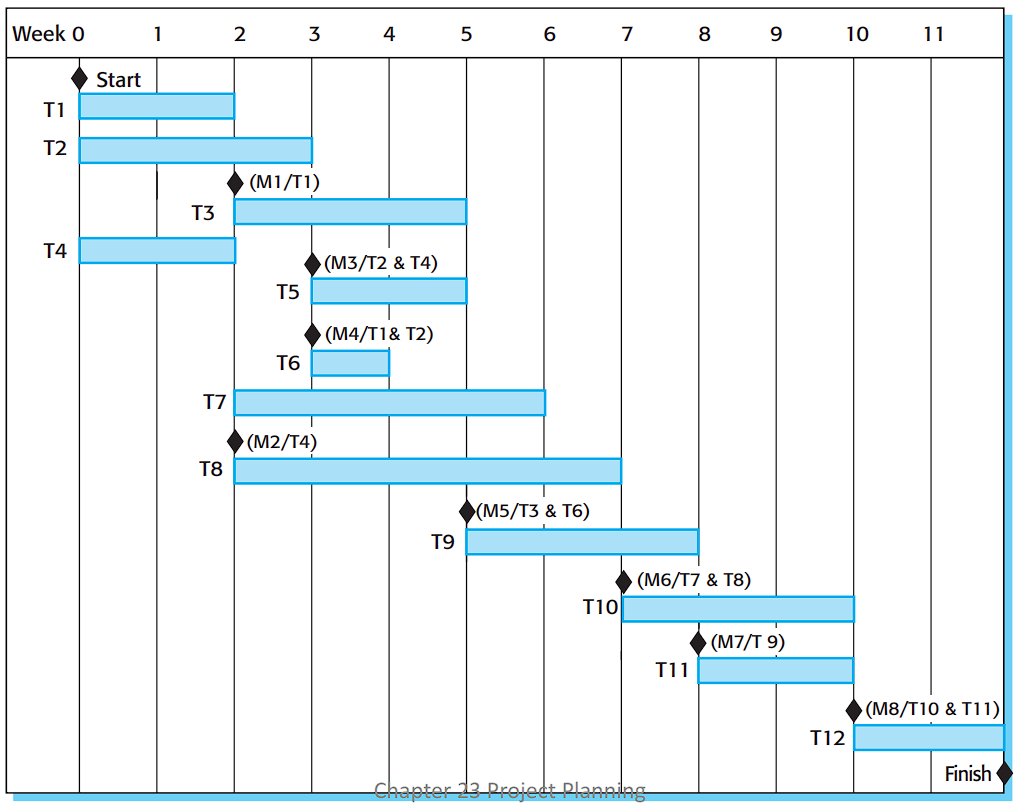
\includegraphics[width=0.45\textwidth ]{images/barChart.png} &
        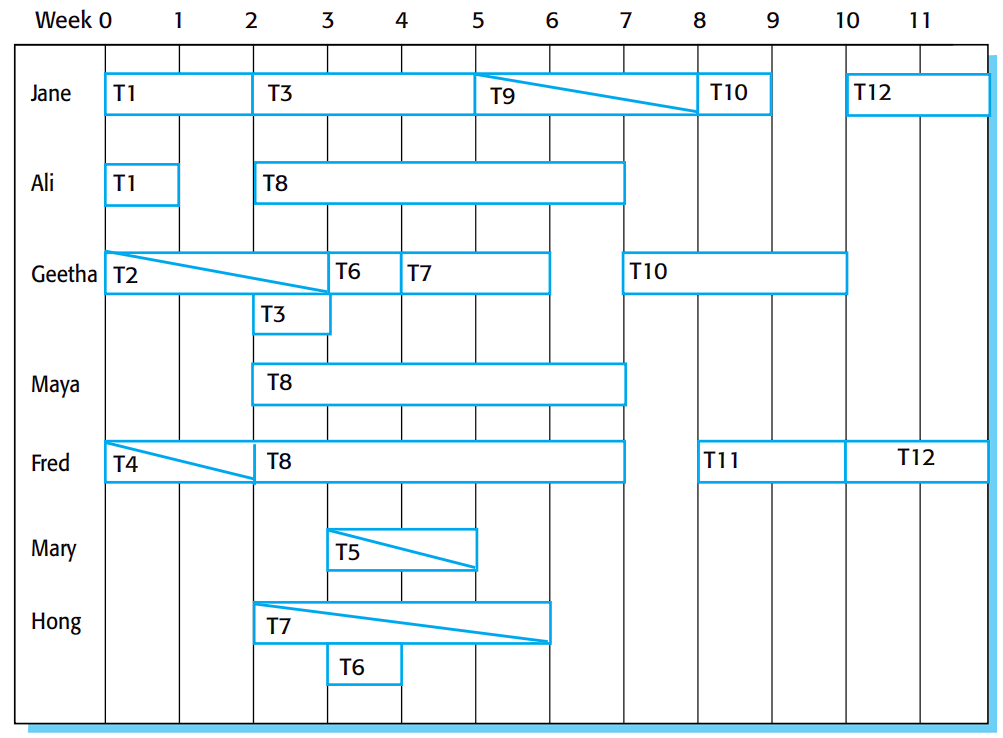
\includegraphics[width=0.5\textwidth ]{images/staffChart.png}
	\end{tabular}
\end{center}
Un \textit{activity bar chart} è un diagramma in cui sull'asse temporale vengono rappresentate 
le varie attività ed il loro scheduling, in modo che le varie dipendenze siano rispettate.\acc 
Analogamente, uno \textit{staff allocation chart} mostra la distribuzione del personale 
suddiviso nelle varie settimane, indicando il progetto alla quale lavorano.\flowerLine 
\section{Sviluppo Agile}
Con sviluppo agile, si denota una metodologia di approccio iterativa in cui il processo di sviluppo ed i 
requisiti vengono rimodellati dinamicamente, in quanto il progetto in fase di sviluppo viene 
considerato dal cliente prima del suo completamento. Diversamente dallo sviluppo plan driven, 
questo approccio non è predeterminato e le decisioni vengono prese durante lo sviluppo, 
possibile aggiunte o rimozioni dipendono da come il progetto procede e dalle nuove priorità del 
cliente.\begin{quote}
    Le priorità e le esigenze del cliente cambiano, quindi ha senso avere un piano flessibile che possa accogliere questi cambiamenti.
\end{quote}
Lo sviluppo agile prevede due stadi\begin{itemize}
    \item \textit{Release planning} : prevede la pianificazione a lungo termine 
    delle funzionalità che dovranno essere implementate nei mesi a venire.
    \item \textit{Iteration planning} : ci si concentra sugli incrementi a breve termine del 
    sistema, tipicamente si tratta di aggiunte che richiedono dalle 2 alle 4 settimane.
\end{itemize}
Una delle metodologie dello sviluppo agile è la 
 pianificazione basata su storie (\textbf{story-based planning}). 
 Consiste nel suddividere le funzionalità di un sistema in piccole unità chiamate 
 "storie utente" (\textit{user stories}). In particolare, sono previsti i seguenti step\begin{enumerate}
    \item Creazione delle storie: Le storie utente sono brevi descrizioni 
    di una funzionalità del sistema dal punto di vista dell'utente finale. 
    Solitamente seguono un formato semplice: "Come utente, voglio [azione] in modo
     da [obiettivo]".
     \item Stima dello sforzo: Il team di sviluppo stima 
     il tempo necessario per implementare ciascuna storia, 
     assegnandole un valore numerico (effort points) che riflette 
     la complessità e la dimensione della storia.
     \item Prioritizzazione: Le storie vengono ordinate in base alla priorità, tenendo 
     conto di fattori come il valore commerciale, l'urgenza e le dipendenze.
     \item Pianificazione delle iterazioni: Le storie prioritarie vengono 
     raggruppate in iterazioni (sprint) di durata definita.
     \item Misurazione della velocità: Viene calcolata la "velocità" del team, 
     ovvero la quantità di lavoro
      (misurata in effort points) che il team riesce a completare in un'iterazione.
      \item Previsione: Sulla base della velocità, il team può stimare il tempo totale 
      necessario per completare il progetto.
 \end{enumerate}
\begin{center}
    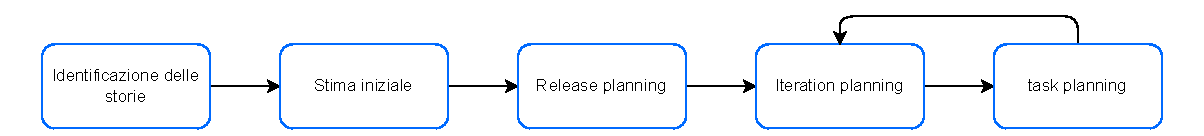
\includegraphics[width=1\textwidth ]{images/planningGame.pdf}
\end{center}
Il  Release Planning si occupa di selezionare e raffinare le storie utente 
(features) che verranno implementate in una specifica versione (release) del prodotto. 
Questo processo definisce quali funzionalità saranno incluse nel rilascio e l'ordine in cui 
verranno sviluppate.\acc 
L'Iteration planning si concentra sulla scelta delle storie utente che verranno implementate 
in ciascuna iterazione (spesso chiamate sprint), che sono periodi di tempo fissi 
(solitamente 2 o 3 settimane) durante i quali il team si impegna a completare un
 insieme di lavoro. Il numero di storie scelte per ogni iterazione dipende dalla capacità del 
team (velocità) di completare il lavoro.\acc 
Durante la fase di pianificazione dei task, gli sviluppatori suddividono le 
storie utente in compiti di sviluppo più piccoli.\begin{itemize}
    \item Un task di sviluppo dovrebbe richiedere tra le 4 e le 16 ore.
    \item Tutti i task necessari per completare tutte le storie di quell'iterazione vengono elencati.
    \item I singoli sviluppatori si offrono volontari per i task specifici che desiderano implementare.
\end{itemize}
Benefici di questo approccio:
\begin{itemize}
    \item L'intero team ha una visione d'insieme dei task da completare in un'iterazione.
    \item Gli sviluppatori si sentono responsabili dei loro task e questo li motiva a completarli.
\end{itemize}
Un incremento del software\footnote{
    un incremento del software rappresenta una porzione funzionante
     e valutabile del prodotto software che viene consegnata alla fine di ogni iterazione
} viene sempre consegnato alla fine di ogni iterazione del progetto.
Se le funzionalità da includere nell'incremento non possono essere completate nel tempo
 previsto, si riducono gli obbiettivi prefissati del lavoro, ma
la tempistica di consegna non viene mai prolungata.\acc
Svantaggi dell'agile planning\begin{itemize}
    \item La pianificazione Agile dipende fortemente 
    dal coinvolgimento e dalla disponibilità del cliente.
    \item può essere difficile da organizzare, poiché i  clienti devono spesso dare priorità ad
     altro lavoro e non sono sempre disponibili per le sessioni di pianificazione.
     \item alcuni clienti potrebbero essere più abituati ai piani di progetto tradizionali e trovare 
     difficile partecipare a un processo di pianificazione agile.
\end{itemize}
La pianificazione agile funziona bene con team di sviluppo piccoli e stabili che 
possono riunirsi e discutere le storie da implementare.
Tuttavia, quando i team sono grandi e/o geograficamente distribuiti, o quando
 la composizione del team cambia frequentemente, è praticamente impossibile coinvolgere
  tutti nella pianificazione collaborativa che è essenziale per la gestione agile di un progetto.
\begin{quote}
    Lo sviluppo agile è un approccio molto efficace per 
    team piccoli e coesi, richiede adattamenti e strumenti specifici 
    per funzionare bene in contesti più grandi e complessi.
\end{quote}
\chapter{Processi Software}
\section{Definizione e Modelli}
\defi{}  Il processo software è un insieme strutturato di attività necessarie per 
sviluppare un sistema software.
Esistono diversi processi software, ma tutti coinvolgono specifiche, progettazione e 
implementazione, validazione ed evoluzione del sistema per rispondere ai bisogni dei clienti.\acc 
Quando descriviamo e discutiamo di processi, di solito parliamo delle attività che 
li compongono, ad esempio, la specifica di un modello di dati, 
la progettazione dell'interfaccia utente, ecc., e dell'ordine in cui queste attività vengono eseguite.
Le descrizioni dei processi possono includere anche:\begin{itemize}
    \item Prodotti: ovvero i risultati di un'attività del processo;
    \item Ruoli: che riflettono le responsabilità delle persone coinvolte nel processo;
    \item Pre-condizioni e post-condizioni: ossia affermazioni che sono vere prima e dopo che un'attività del processo è stata eseguita o un prodotto è stato creato.
\end{itemize}
Come già accennato, i processi software possono essere di due tipi\begin{itemize}
    \item \textbf{processi plan-driven} : Sono processi in cui tutte le attività vengono
     pianificate in anticipo e l'avanzamento del progetto viene misurato in base a 
     questo piano iniziale. È come seguire una ricetta precisa, dove ogni passo è 
     definito fin dall'inizio 
     \item \textbf{processi agili} : In questi processi, la pianificazione è più flessibile
      e si adatta ai cambiamenti. Si lavora a iterazioni brevi (sprint) e si può modificare 
      il piano di volta in volta in base alle nuove esigenze del cliente. È come cucinare 
      senza una ricetta precisa, ma adattando i piatti ai gusti degli ospiti man mano che 
      si procede.
\end{itemize}
Nella pratica La maggior parte dei progetti software combina elementi di entrambi gli approcci. A volte è necessario un piano dettagliato per le fasi iniziali, mentre in altre si può essere più flessibili.\acc 
Il processo software vive attraverso differenti formulazioni, o \textit{modelli}, precisamente verranno trattati i seguenti\begin{itemize}
    \item \textit{waterfall model} 
    \item \textit{incremental development}
    \item \textit{integration and configuration}
\end{itemize}
Nella pratica, i sistemi di grandi dimensioni incorporano elementi da più modelli.
\subsubsection{Waterfall Model}
È uno dei modelli di sviluppo software più antichi e tradizionali è di tipo plan driven e consiste nell'individuare e separare le distinte fasi di  
specifica e sviluppo. Tali fasi sono\begin{itemize}
    \item analisi e definizione dei requisiti 
    \item progettazione del sistema e del software 
    \item implementazione e collaudo 
    \item integrazione e deployment del sistema 
    \item mantenimento
\end{itemize}
Gli svantaggi di tale modello risiedono nella poca flessibilità e robustezza nell'accomodare 
richieste di cambiamento una volta che il progetto è indirizzato su una certa via. 
Generalmente, è necessario terminare una fase prima di passare alla successiva.
\begin{figure}[h!]
    \centering 
    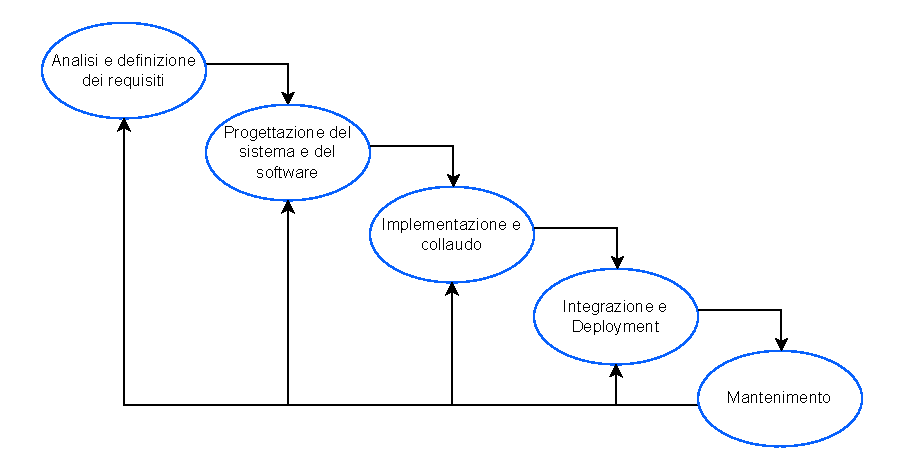
\includegraphics[width=0.7\textwidth ]{images/waterfallModel.pdf}
    \caption{Il modello waterfall}
\end{figure}
Il modello a cascata divide il progetto in fasi distinte e rigide, rendendo difficile adattarsi ai cambiamenti nei requisiti del cliente.\begin{itemize}
    \item Limitazioni nei requisiti: Questo modello è adatto solo quando i requisiti sono ben definiti all'inizio del progetto e non si prevedono grandi modifiche durante lo sviluppo.
    \item Instabilità dei requisiti: Nella maggior parte dei casi, i requisiti dei sistemi informatici non sono statici, ma cambiano nel tempo.
\end{itemize}
Il modello a cascata viene spesso utilizzato in progetti di ingegneria software su larga scala, dove il sistema viene sviluppato in più sedi.  In questi casi, la natura pianificata del modello a cascata aiuta a coordinare le attività tra i diversi team di sviluppo.
\subsubsection{Incremental Development}
Tale modello di \textit{sviluppo incrementale} punta alla riduzione dei costi necessari per 
accomodare le nuove richieste del cliente che insorgono a progetto già avviato. La quantità di analisi e documentazione da rifare è molto inferiore rispetto al modello a cascata : si riduce la necessità di ricominciare da capo se i requisiti cambiano, risparmiando tempo e risorse. 
\begin{itemize}
    \item \textit{È più facile ottenere feedback dal cliente sul lavoro di sviluppo svolto} : Il cliente può vedere e provare il software in fase di sviluppo e fornire un feedback diretto, contribuendo a migliorare il prodotto finale. 
    \item \textit{È possibile una consegna e un deployment più rapidi del software utile per il cliente} : Il cliente può iniziare a utilizzare il software prima rispetto al modello a cascata, ottenendo così un beneficio più rapido dal prodotto.
\end{itemize}\begin{center}
\begin{figure}[h!]
    \centering 
    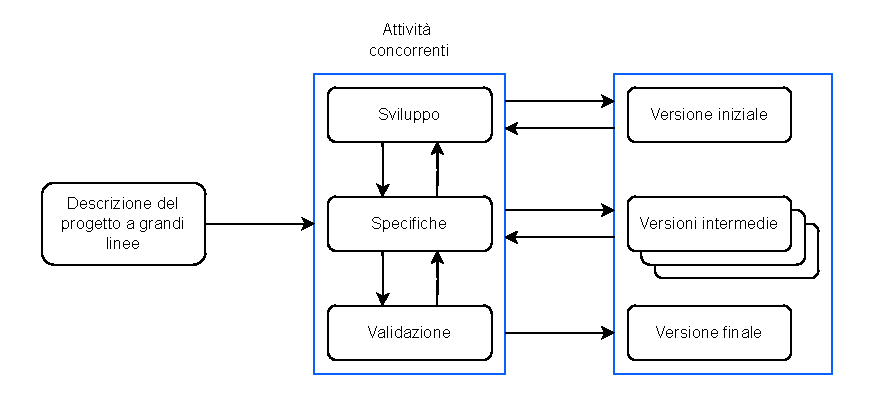
\includegraphics[width=0.8\textwidth ]{images/IncrementalDevelopment.pdf}
    \caption{Incremental Development}
\end{figure}\end{center}
Il modello comporta alcuni svantaggi\begin{itemize}
    \item \textbf{Mancanza di visibilità per i manager}: I manager spesso necessitano di deliverable regolari per misurare l'avanzamento del progetto. In uno sviluppo incrementale rapido, produrre documentazione dettagliata per ogni versione può risultare costoso e inefficiente. La natura iterativa dello sviluppo incrementale può rendere complesso tracciare tutti i cambiamenti apportati al sistema nel tempo.
    \item \textbf{Degradazione della struttura del sistema}: L'aggiunta continua di nuove funzionalità senza una adeguata manutenzione può portare al degrado della struttura del codice, rendendolo più complesso e meno manutenibile. Man mano che il sistema cresce, diventa sempre più difficile apportare modifiche senza introdurre nuovi bug o impatti negativi su altre parti del sistema.
\end{itemize}
\subsubsection{Integration and configuration}
È un modello basato sul riutilizzo del software: I sistemi vengono costruiti combinando componenti software preesistenti o sistemi applicativi già pronti all'uso (spesso chiamati COTS - Commercial-off-the-shelf). Spesso avviene una riconfigurazione degli elementi riutilizzati, tali componenti possono essere personalizzati per adattarsi alle specifiche esigenze dell'utente. \acc Il riutilizzo del software è diventato il metodo più comune per sviluppare molti tipi di sistemi aziendali, verrà trattato approfonditamente in seguito. Esistono diversi tipi di \textbf{software riutilizzabile}\begin{itemize}
    \item Sistemi applicativi autonomi (a volte chiamati COTS) che vengono configurati per l'uso in un ambiente specifico.
    \item Collezioni di oggetti sviluppati a mò di pacchetto da integrare in un framework di componenti come .NET o J2EE. 
    \item Servizi web sviluppati secondo standard e disponibili per essere integrati remotamente.
\end{itemize}
Le fasi chiave del processo sono\begin{enumerate}
    \item Specifica dei requisiti 
    \item Definizione e valutazione del software 
    \item Raffinamento dei requisiti 
    \item Configurazione del sistema 
    \item Adattamento e integrazione dei componenti
\end{enumerate}
Vantaggi\begin{itemize}
    \item Costi e rischi ridotti, poiché si sviluppa meno software da zero 
    \item Consegna e implementazione più rapida del sistema
\end{itemize}
Svantaggi\begin{itemize}
    \item  sono inevitabili dei compromessi sui requisiti, quindi il sistema potrebbe non soddisfare pienamente le esigenze degli utenti 
    \item Perdita di controllo sull'evoluzione degli elementi del sistema riutilizzati, Non avendo il controllo completo sul codice sorgente dei componenti riutilizzati
\end{itemize}
\begin{center}
    \begin{figure}[h!]
        \centering 
        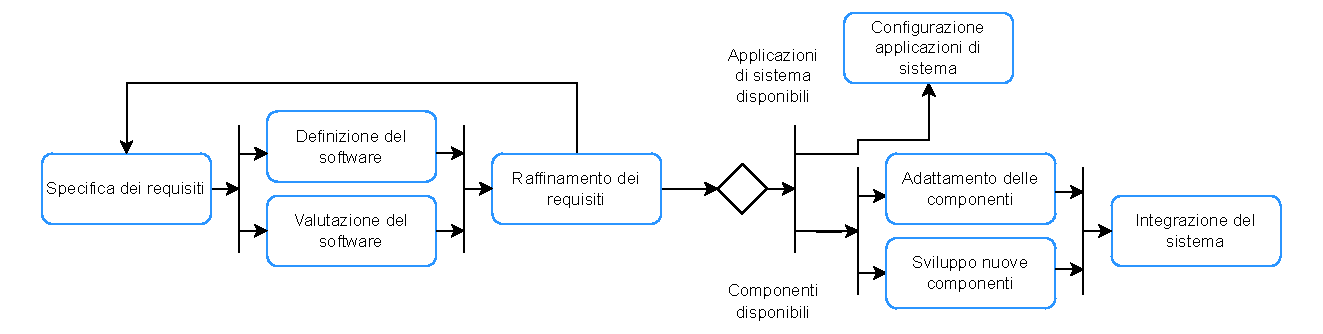
\includegraphics[width=1\textwidth ]{images/IngegneriaRiuso.pdf}
        \caption{Ingegneria del software orientata al riciclo}
    \end{figure}\end{center}
\end{document}